\documentclass[12pt]{report}

\usepackage[left=1in, right=1in, top=1in, bottom=1in]{geometry}
\setlength\parindent{0pt}

\usepackage{graphicx, amsmath,anonchap,tabularx, multicol,verbatim}

\usepackage{enumitem}
\setlist{noitemsep}
\setlist{nolistsep}

\newenvironment{boxe}
    {\begin{center}
    \begin{tabular}{|p{0.9\textwidth}|}
    \hline\\
    }
    { 
    \\\\\hline
    \end{tabular} 
    \end{center}
    }

\begin{document}

\begin{tabular*}{\textwidth}{@{\extracolsep{\fill}}ll}
\textbf{One Sided Limits}  & Name: \rule{6cm}{0.5pt} \\
MATH 160 & Section:\hspace{1in} \\
\hline\hline
\end{tabular*} \\

\pagenumbering{gobble}

\sf
\textbf{Learning Targets:}
\begin{itemize}
\item Evaluate one-sided limits graphically and algebraically.				
\item Use information about the one-sided limits to infer the existence or non-existence of a (two-sided) limit.
\item Reframe functions with absolute values using piecewise-defined functions and evaluate limits.
 \end{itemize}
Aligns with Standard L2. \rm

\hrulefill 

\subsection*{One Sided Limits}

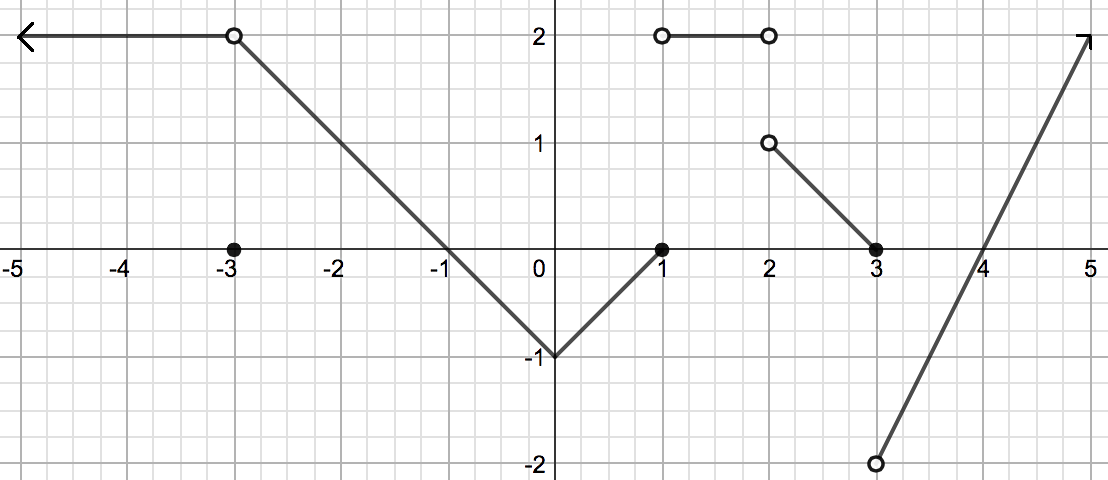
\includegraphics[scale=0.75]{2_4_pic1.png}
%\bigskip

\begin{multicols}{3}
\begin{enumerate}[parsep=.25in]

\item $\displaystyle\lim_{x\rightarrow-3^-}f(x)=$ 
\item $\displaystyle\lim_{x\rightarrow-3^+}f(x)=$
\item $\displaystyle\lim_{x\rightarrow-3}f(x)=$ 
\item $\displaystyle\lim_{x\rightarrow0^-}f(x)=$ 
\item $\displaystyle\lim_{x\rightarrow0^+}f(x)=$ 
\item $\displaystyle\lim_{x\rightarrow0}f(x)=$ 
\item $\displaystyle\lim_{x\rightarrow2^-}f(x)=$ 
\item $\displaystyle\lim_{x\rightarrow2^+}f(x)=$ 
\item $\displaystyle\lim_{x\rightarrow2}f(x)=$ 
\item $\displaystyle\lim_{x\rightarrow3^-}f(x)=$ 
\item $\displaystyle\lim_{x\rightarrow3^+}f(x)=$ 
\item $\displaystyle\lim_{x\rightarrow3}f(x)=$ 
\item $\displaystyle\lim_{x\rightarrow4^-}f(x)=$ 
\item $\displaystyle\lim_{x\rightarrow4^+}f(x)=$ 
\item $\displaystyle\lim_{x\rightarrow4}f(x)=$ 
\end{enumerate}

\bigskip
\bigskip
Let's also compute some function values:

\bigskip

\begin{enumerate}[parsep=.1in]
\item $f(-3)=$
\item $f(0)=$
\item $f(1)=$
\item $f(2)=$
\item $f(3)=$
\item $f(4)=$
\end{enumerate}
\end{multicols}

\subsubsection*{A Consequence of One Sided Limits}
What do you notice about the connection between the one sided limits 
$\displaystyle\lim_{x\rightarrow c^-}f(x)$, $\displaystyle\lim_{x\rightarrow c^+}f(x)$ 
and the full limit $\displaystyle\lim_{x\rightarrow c}f(x)$?
\\\\\\\\\\\\\\\\\\\\\\\\\\

\section*{Rewriting}
How can $f(x)=|x|$ be written as a piecewise function?

\bigskip

$f(x)=\begin{cases} \underline{\hspace{1in}} &  \underline{\hspace{1in}} \\ \underline{\hspace{1in}} & \underline{\hspace{1in}} \end{cases}$

\bigskip
How can $g(x)=|x+4|$ be written as a piecewise function?

\bigskip

$g(x)=\begin{cases} \underline{\hspace{1in}} &  \underline{\hspace{1in}} \\ \underline{\hspace{1in}} & \underline{\hspace{1in}} \end{cases}$

\bigskip
How can $h(x)=\displaystyle\frac{|2-x|}{x}$ be written as a piecewise function?

\bigskip

$h(x)=\begin{cases} \underline{\hspace{1in}} &  \underline{\hspace{1in}} \\ \underline{\hspace{1in}} & \underline{\hspace{1in}} \end{cases}$


\end{document}
